\section{Introduction}
% Autonomous agents that interact with an environment usually face tasks  that comprise complex, entangled behaviors over long horizons. Conventional reinforcement learning (RL) methods have successfully addressed this. Notwithstanding, there are cha  However, a common scenario in RL is that where the agent performs several tasks (which are specified by different reward functions) across similar environments, where the dynamics remain the same but the reward function changes. Training a policy for every task separately is time-consuming and requires a lot of data. In such cases, the agent can utilize a method that has built-in generalization capabilities. One such method relies on the assumption that reward function of these tasks can be decomposed into a linear combination of some feature map~\citep{Barreto2017}. When a new task is presented, it is possible to combine previously learned policies and their successor features to solve a new task. %While the combination of such policies is guaranteed to be better than any previously learned policy, it need not be optimal.
% While combining such policies is guaranteed to be an improvement over any previously learned policy, it may not necessarily be optimal. 

Autonomous agents that interact with an environment usually face tasks that comprise complex, entangled behaviors over long horizons. Conventional reinforcement learning (RL) methods have successfully address this. Notwithstanding, there are some limitations that are inherent to classical RL methods, even when they are endowed with function approximation techniques. One of such challenges is that stadard RL algorithms are data greedy and training tasks from scratch is usually inefficient. In this line, there is no universal consensus about how to combine previously learned behaviors so the combined policy generalizes predictably to unseen tasks. As it was introduced in section~\ref{section:successor_features}, the successor features framework is a way to allow generalization in the context of RL. Nonetheless, the question of identifying which policies should be in the so-called basis was up to this point unclear, leaving the problem of optimal policy transfer open. Another challenge is that traditional RL methods rely on Markovian reward functions. Section~\ref{section:non_markovian} describes cases where coming up with these reward specification might be difficult or even not possible at all. In such scenarios, there has been a growing interest in alternative methods for non-Markovian task specification in recent years. The work of~\citet{Camacho2019} and~\citet{Icarte2022} purveyed techniques that successfully use formal languages for such specifications. 

%While these and other conventional RL methods use Markovian reward functions, expressing a task with such reward function can be difficult and may not even be possible in some cases~\citep{Whitehead1995}. In settings where the reward function cannot be expressed in Markovian terms, task specification has raised especial interest in the last few years~\citep{Icarte2022, Camacho2019}.

The method introduced in this chapter aims to build optimal solutions to non-Markovian reward functions exploiting the generalization capabilities of successor features. In this context, prior techniques for tackling similar problems have been proposed. As it was explained in section~\ref{section:non_markovian}, a fundamental assumption in this setting is there exist a set of propositional symbols that permits the definition of high-level tasks using logic~\citep{ToroIcarte2019, Vaezipoor2021} or finite state automata (FSA)~\citep{Icarte2022}. This field is tightly connected to hierarchical RL. This connection arises naturally when satisying subtaks is seen as solving a problem in isolation, which can be then combined for a global solution in the high-level. However, combining optimal solutions for subtasks may potentially result in a suboptimal overall policy, and many of these approaches produce \textit{myopic policies}~\citep{Vaezipoor2021} (whcih are equivalent to recursively optimal policies in the context of hierarchical RL).

More broadly, generalization has been introduced by conditioning the policy or the value function on the specification of the whole task~\citep{Schaul2015}. Such approaches were recently also proposed for tasks with non-Markovian reward functions \citep{Vaezipoor2021}. However, the methods that specify the whole task usually rely on a blackbox neural network for planning when determining which subgoal to reach next. This makes it hard to interpret the plan to solve the task and although they show promising results in practice, %they achieve promising empirical results 
it is unclear whether and when these approaches will generalize to a new task. 

 % In this case, it is also possible to simplify the task description once a subgoal has been achieved to improve the data efficiency and generalization. 
Instead, this chapter describes a method that uses task descomposition without sacrifing the global optimality of the solution while at the same times attains predictable generalization. The derived approach, \textsc{sf-fsa-vi}, is a two-stage algorithm in which (i) a set of \textit{local} (sub)policies are learned for a specific choice of a feature representation and (ii) this set of policies is used in a planning step to retrieve the optimal solution to any problem that can be described with an FSA, without additional learning.

\section{Contributions}
More specifically, this work makes the following contributions
 \begin{itemize}
    \item To use successor features to learn a policy basis that is suitable for planning even in stochastic domains.
    \item To provide a planning framework that uses such policy bases for zero-shot generalization to complex temporal tasks described by an arbitrary FSA.
    \item To prove that if the policies in this basis are optimal, this framework produces a globally optimal solution even in stochastic domains.
    \item To provide empirical results that demonstate the improvement over other baselines.
\end{itemize}

\section{Preliminaries}

In this section we set the ground for our method. The subsequent paragraphs describe the relationship of the building blocks of the method, namely the FSA task specification, the feature vectors, and the policy basis for the low-level.

Our method assumes that the low-level is modeled by a family of MDPs (see section~\ref{section:successor_features})
\begin{equation}
  \cM^{\boldsymbol{\phi}}\equiv\{\langle\cS,\cE,\cA,\cR_\w,\mathbb{P}_0, \mathbb{P},\gamma\rangle \lvert \cR_\w = \w^\intercal \boldsymbol{\phi}, \forall\w\in\real^d\},
\end{equation}
where there is a propositonal vocabulary $\cP$ that relates to the feature map $\boldsymbol{\phi}$ and the set of exit states $\cE$. 

\paragraph{Propositional Logic} Environments are assummed to be endowed with a set of high-level, boolean-valued propositional symbols $\cP$. Wihtout loss of generality, it is assumed that these symbols are observed when the agent transitions into some exit state $\varepsilon\in\cE$ of the low-level MDP $\cM^{\boldsymbol{\phi}}$, though this may not be the case. Every transition $(s, a, s')\in\cS\times\cA\times\cS$ induces some propositional valuation (assignment of truth values) $2^\cP$. Such a valuation depends solely on the new state $s'$ and occurs under a mapping ${\cO:\cS\rightarrow2^\cP}$ that is known to the agent. This implies that the agent can associate valuations $2^\cP$ to transitions at every moment. Propositional symbols are assumed to be mutually exclusive, and the agent cannot observe two symbols evaluated with true in the same transition. A valuation $\Gamma$ is said to satisfy a propositional symbol $p$, formally $\Gamma\vDash p$, if $p$ is true in $\Gamma$. 

\paragraph{Finite State Automaton} High-level tasks are instructed via finite state automata. These are tuples ${\cF=\langle \cU,u_0,\cT,L,\delta\rangle}$ where $\cU$ is the finite set of states, $u_0\in\cU$ is the initial state, $\cT$ is the set of terminal states with $\cU\cap\cT=\emptyset$, $L:\cU\times(\cU\cup\cT)\rightarrow 2^\cP$ is a labelling function that maps FSA states transitions to truth values for the propositions and $\delta:\cT\rightarrow \real$ is a high-level reward function for terminal states. Each transition among FSA states $(u, u')$ defines a subgoal. The agent has to observe some propositional valuation $L(u, u')$ in order to achieve it and FSA states can only be connected by a subgoal. E.g., in Figure~\ref{fig:office_fsa}, the FSA state $u_0$ has two outgoing subgoals: getting mail (labeled as \mail) and getting coffee (labeled as \coffee). Non-existing transitions $(u, u')$ get mapped to $L(u, u')=\bot$. The reward function $\delta$ gives a reward only to terminal states. %In other words, such a reward function is $\delta(u)=0\;\forall u\in\cU$ and $\delta(\mathbf{t})=1\;\forall \mathbf{t}\in\cT$. 


\begin{figure}[!tb]
  \centering
  \begin{subfigure}[h]{0.5\textwidth}
    \centering
  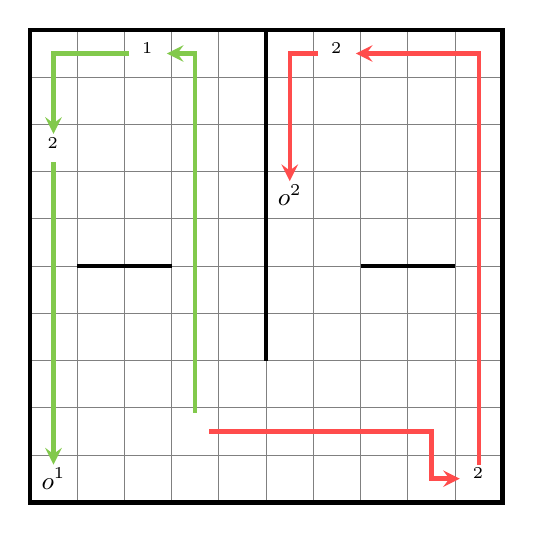
\begin{tikzpicture}[scale=0.6]
    % grid
    \draw[step=1cm,gray] (0,0) grid (10, 10);
    % walls
    \draw[ultra thick, fill=black] (5,10) -- (5, 3);
    \draw[ultra thick, fill=black] (1,5) -- (3, 5);
    \draw[ultra thick, fill=black] (7,5) -- (9, 5);

    % Symbols
    \node at (0.5,0.5) {\small $o^1$};
    \node at (0.5,7.5) {\small $\text{\mail}^2$};
    \node at (2.5,9.5) {\small $\text{\coffee}^1$};
    \node at (6.5,9.5) {\small $\text{\coffee}^2$};
    \node at (5.5,6.5) {\small $o^2$};
    \node at (9.5,0.5) {\small $\text{\mail}^2$};

    % agent
    \node at (3.5,1.5) {\small \agent};
    % Optimal path
    \draw[ultra thick, ->, >=stealth, draw=green!70!red!70] (3.5,1.9) -- (3.5,9.5) -- (2.9,9.5);
    \draw[ultra thick, ->, >=stealth, draw=green!70!red!70] (2.1,9.5) -- (0.5,9.5) -- (0.5,7.8) ;
    \draw[ultra thick, ->, >=stealth, draw=green!70!red!70] (0.5,7.2) -- (0.5,0.8);
    % Suboptimal path
     \draw[ultra thick, ->, >=stealth, draw=red!70!white] (3.8, 1.5) -- (8.5, 1.5) -- (8.5, 0.5) -- (9.1, 0.5);
     \draw[ultra thick, ->, >=stealth, draw=red!70!white] (9.5, 0.8) -- (9.5, 9.5) -- (6.9, 9.5);
     \draw[ultra thick, ->, >=stealth, draw=red!70!white] (6.1, 9.5) -- (5.5, 9.5) -- (5.5, 6.8);
    % \draw[ultra thick, ->, >=stealth, draw=blue!70!white] (2.5,1.9) -- (2.5,2.5) -- (1.5,2.5) -- (1.5,3.5) -- (2.5,3.5) -- (2.5,5.5) -- (1.5,5.5) -- (1.5,6.5) -- (2.5,6.5) -- (2.5,7.5) -- (3.5,7.5) -- (3.5,6.8);
    % \draw[ultra thick, ->, >=stealth, draw=blue!70!white] (3.8,6.5) -- (4.3,6.5) -- (4.3,4.8);

    % Outer box
    \draw[ultra thick] (0,0) rectangle (10,10);

\end{tikzpicture}


  \subcaption{}
  \label{fig:office_env}
  \end{subfigure}
  \hfill
  \centering
  \begin{subfigure}[h]{0.49\textwidth}
    \centering
  \begin{tikzpicture}[node distance=cm,on grid,every initial by arrow/.style={ultra thick,->, >=stealth}]
    \node[thick,state,initial above] (u_0) at (0,0) {$u_0$};
    \node[thick,state]         (u_1) at (-1.5, -1.4)  {$u_1$};
    \node[thick,state]         (u_2) at (1.5, -1.4)  {$u_2$};
    \node[thick,state]         (u_3) at (0, -2.9)  {$u_3$};

    \node[circle,draw=black,minimum size=0.26cm,inner sep=0pt,fill=black] (t3) at (0,-4.3)  {};
    \node[text width=1cm ] at (0.7, -4.2) {$u_T$};

    \path[thick,->, >=stealth] (u_0) edge node [left] {$\text{\coffee}$} (u_1);
    \path[thick,->, >=stealth] (u_0) edge node [right] {$\text{\mail}$} (u_2);
    \path[thick,->, >=stealth] (u_1) edge node [left] {$\text{\mail}$} (u_3);
    \path[thick,->, >=stealth] (u_2) edge node [right] {$\text{\coffee}$} (u_3);
    \path[thick,->, >=stealth] (u_3) edge node [left] {$\text{o}$} (t3);
    
    %\path[ultra thick,->, >=stealth] (q_0) edge [loop left] node {$\tuple{\neg \text{\coffee},0}$} ();
    % \path[ultra thick,->, >=stealth] (q_0) edge node [above] {$\tuple{\text{\decoration},0}$} (t1);
    %\path[ultra thick,->, >=stealth] (q_1) edge [loop left] node {$\tuple{\neg o,0}$} ();
    % \path[ultra thick,->, >=stealth] (q_1) edge node [above] {$\tuple{\text{\decoration},0}$} (t2);
    %\path[ultra thick,->, >=stealth] (u_1) edge node [above]{$o$} (t3);
\end{tikzpicture}
  \subcaption{}
  \label{fig:office_fsa}
  \end{subfigure}
  \caption{(a) Depiction of the Office environment. The propositional symbols are $\cP=\{\text{\coffee}, \text{\mail}, o\}$ while the set of exit states is $\cE=\{\text{\coffee}^1,\text{\coffee}^2, \text{\mail}^1,\text{\mail}^2, o^1, o^2\}$. The red and green paths show a suboptimal and optimal (resp.) trajectories for the task `get coffee and mail in any order, then go to an office location' whose FSA is represented in (b).}
\end{figure}

\paragraph{Feature vectors} For a family of MDPs $\cM^{\boldsymbol{\phi}}$, the feature map is ${\boldsymbol{\phi}}:\cS\times\cA\times\cS\rightarrow\real^{\lvert\cE\rvert}$. Each feature component $\boldsymbol\phi_j$ is associated with an exit state $\varepsilon_j\in\cE=\{\varepsilon_1,\ldots,\varepsilon_{\lvert\cE\rvert}\}$. Such vectors are built as follows. At terminal transitions $(s, a, \varepsilon_i)\in T$, $\boldsymbol\phi_{j} = 1$ when $j=i$ and $\boldsymbol\phi_{j}=0$ when $j\neq i$. For non-terminal transitions, it is just required that $\w^\intercal\boldsymbol\phi(s, a, s')<1$. In the case that ${\boldsymbol\phi(s, a, s')=\mathbf{0}\in\real^{\lvert\cE\rvert}}$, the SF representation in Equation~\eqref{eq:sf} of each policy consists of a discounted distribution over the exit states. This indicates how likely it is to reach each exit state following such a policy. Furthermore, it is required that $\cE\subset\text{supp}(\mathbb{P}_0)$ so the value functions at exit states are well-defined. Additionally, one can consider extra symbols in $\cP$ that are not necessarily satisfied at the exit states. Think, for example, about a propositional symbol $q\in\cP$ that represents an obstacle which has a penalty effect. In such cases, the feature vector can be extended to be of dimension $\lvert\cE\rvert + 1$, where the extra component is $-1$ when $q$ is observed, and $0$ otherwise. 

\paragraph{Policy basis and convex coverage set} The recent work of~\citep{Alegre2022} solves the optimal policy transfer learning problem. They draw the connection between the SF transfer learning problem and multi-objective RL (MORL). The pivotal fact is that the SF representation in Equation~\eqref{eq:sf} can be interpreted as a multidimensional value function and the construction of the aforementioned set of policies $\Pi$ can be cast as a multi-objective optimization problem.
 
 Consequently, the optimistic linear support (OLS) algorithm is extended with successor features in order to learn a set of policies that constitutes a \textit{convex coverage set} (CCS)~\citep{Roijers2015}. Their main result is the SFOLS algorithm (see Supplementary Material\footnote{Supplementary Material at {\texttt{\url{https://arxiv.org/abs/2403.15301}}}} for a full, technical description) in which a set $\Pi_\text{CCS}$ is built incrementally by adding (new) policies to such a set, until convergence. The set $\Pi_\text{CCS}$ contains all non-dominated policies in terms of their multi-objective value functions, where the dominance relation is defined over scalarized values ${V^\pi_\w = \mathbb{E}_{S_0\sim\mathbb{P}_0}\left[V^\pi_\w(S_0)\right]}$, and is characterized as
\begin{align}
  \Pi_\text{CCS} &= \{\pi\;\lvert\;\exists\w\;\text{s.t.}\;\forall {\boldpsi}^{\pi'},\; \w^\intercal {\boldpsi}^\pi {\;\geq\;} \w^\intercal{\boldpsi}^{\pi'} \} \nonumber\\
  &= \{ \pi \;\lvert\;\exists\w\;\text{s.t.}\;\forall {\pi'},\; {V^\pi_\w}{\;\geq\;} {V^{\pi'}_\w}\}.
\end{align} 
In every iteration $k$, SFOLS proposes a new weight vector $\w^k\in\Delta(d)$ for which an optimal policy (and its corresponding SF representation) is learned and added to $\Pi_\text{CCS}$ since it is sufficient to consider weights in $\Delta(d)$ to learn the full $\Pi_\text{CCS}$. The output of SFOLS is both $\Pi_\text{CCS}$ and the SF representation $\boldpsi^\pi$ for every $\pi\in\Pi_\text{CCS}$.
 
Intuitively, all policies in $\Pi_\text{CCS}$ are optimal in at least one task $\w \in \Delta(d)$.
The set $\Pi_\text{CCS}$ is combined with GPI, see Equation~\eqref{eq:gpi}, and upon convergence, for any (new) given task $\w'\in\real^d$, an optimal policy can be identified~\citep[cf. Theorem 2]{Alegre2022}.


\section{Using Successor Features to Solve non-Markovian Reward Specifications}

\textsc{sf-fsa-vi} focuses on the setting in which a low-level MDP is equipped with a reward structure like in Equation~\eqref{eq:reward_sf}. The low-level is represented by a family of MDPs $\cM^{\boldsymbol{\phi}}$, where each weight vector $\w\in\real^d$ specifies a low-level task. The agent receives high-level task specifications in the more flexible form of an FSA which permits the specification of non-Markovian reward structures. The combination of a low-level family of MDPs and a high-level FSA gives rise to a \textit{product MDP} $\cM'=\cF\times\cM^{\boldsymbol{\phi}}$ that satisfies the Markov property, and where the state space is augmented to be $\;\cU\times\cS$. This product MDP follows the same philosophy as the cross product MDP proposed by \citet{Icarte2022}.

A product MDP $\cM'$ is a well-defined MDP, though in this case the agent now follows a policy $\mu:\cU\times\cS\rightarrow\Delta(\cA)$, that depends on both the FSA state and the underlying MDP state. $\cM'$ can be solved with conventional RL methods such as Q-learning~\citep{Watkins1992} by finding an optimal policy $\mu^*$ that maximizes
\begin{equation*}
Q^\mu(u, s, a) = \EEcp{\sum_{i=t}^\infty \gamma^{i-t}\cR_i}{U_t= u, S_t=s, A_t=a}{\mu}.
\end{equation*}
This is, however, impractical since policies should be retrained every time a new high-level task is specified. Exploiting the problem structure is essential for tractable learning, where components can be reused for new task specifications. The special reward structure of the low-level MDPs and the particular choice of feature vectors, previously introduced, allows definining an algorithm able to achieve a solution by simply planning in the space of augmented exit states $\;\cU\times\cE$. This inherently makes obtaining an optimal policy more efficient than solving the whole product MDP, as the number of states on which it is necessary to compute the high-level value function is drastically reduced.

When presented with different task specifications (e.g.~Figure~\ref{fig:office_fsa}), the agent may have to perform the same subtask at different moments of the plan or in different FSAs. The aim is to provide agents with a collection of base behaviors that can be combined to retrieve the optimal behavior for the whole task.

In line with the previous reasoning, \textsc{sf-fsa-vi} a two-step algorithm in which the agent first learns a $\Pi_{\text{CCS}}$ (a set of policies that constitute a CCS) on a well-specified representation of the environment. Then these (sub)policies are used to solve efficiently any FSA task specification on the propositional symbols of the environment. 

 \paragraph{Example} In the office domain depicted in Figure~\ref{fig:office_env}, the propositional symbols are $\cP=\{\text{\coffee}, \text{\mail}, \text{o}\}$ while the exit states $\cE=\{\text{\coffee}^1, \text{\coffee}^2,\text{\mail}^1,\text{\mail}^2,o^1,o^2\}$. Consequently, the same propositional symbol is satisfied at different exit locations, this is $\cO(\text{\coffee}^1)\vDash\text{\coffee}$ and $\cO(\text{\coffee}^2)\vDash\text{\coffee}$. In this case, $\boldsymbol\phi(s, a, s')\in\real^6$, is defined as the zero vector $\mathbf{0}\in\real^6$ for every $s'\in\cS\setminus\cE$ and gets the corresponding vector component equal to $1$ when $s'\in\cE$. Figure~\ref{fig:office_fsa} the FSA task specification for a `composite' task in this domain, note that FSAs use symbols in $\cP$ to define the subgoals. The natural language interpretation of this FSA is `get coffee and mail in any order, then go to an office'. Figure~\ref{fig:office_env} also shows two different (among multiple possibilities) ways of satisfying such a high-level task. Recursively optimal methods retrieve a suboptimal solution (such as the one in red). Even though this solution satisfies the first subtask in shorter number of steps, the overall solution is longer than the optimal one (in green).

\subsection{Algorithm} 

\begin{algorithm}[!htb]
  \caption{\textsc{sf-fsa-vi}}
  \textbf{Input:} Low-level MDP $\cM^{\boldsymbol{\phi}}$, task specification $\cF$
  \begin{algorithmic}[1]
    \State Obtain $\Pi_\text{CCS}$ on $\cM^{\boldsymbol{\phi}}$.
    \State Initially  $\w^0(u) = \mathbf{0} \in\real^{\lvert\cE\rvert}\;\;\forall u\in\cU$.
   
    \While{not done}
      \For{$u \in \cU$}
        
        \State Update each $\w^{k+1}_j{(u)}$ with Equation~\eqref{eq:update_rule}.
       
      \EndFor
    \EndWhile
    
    \State \Return $\{\w^*(u)\;\forall u\in\cU\}$
  \end{algorithmic}
  \label{alg:online}
\end{algorithm}

The solution to an FSA task specification implies solving a product MDP $\cM'=\cF\times\cM^{\boldsymbol{\phi}}$. Since there is access to the CCS, the optimal Q-function can be represented by a weight vector $\w^*$:
\begin{equation}
    Q^*_\w(u,s,a) = \smashoperator{\max_{\pi\in\Pi_\text{CCS}}} \w^*(u)^{\intercal}\boldsymbol{\psi}^\pi(s,a).
    \label{eq:extended_qfunction}
\end{equation}
for all $(u,s,a)\in\cU\times\cS\times\cA$. Here, $\w_j^*(u)$ indicates the optimal value from exit state $\varepsilon_j\in\cE$ for FSA state $u$. Then an optimal policy is defined as
\begin{equation}
    \mu^*_\w(u, s) \in \argmax_{a\in\cA} Q^*_\w(u,s,a)\;\forall(s,u)\in\cU\times\cS.
    \label{eq:hl-policy}    
\end{equation}
Therefore, a key observation is that that finding the optimal weight vectors $\w^*(u)$, ${\forall u\in\cU}$ is enough for retrieving the optimal action value function of the product MDP $\cM'$ and, thus, an optimal policy.
This vector can be obtained using a dynamic-programming approach similar to value iteration: 
\begin{align}
\w_j^{k+1}(u) =&  \max_a Q^*_\w\bigl(\tau(u,\cO(\varepsilon_j)),a\bigr) \\
              =& 
    \max_{a,\pi} \w^k\bigl(\tau(u,\cO(\varepsilon_j))\bigr)^{\intercal} \boldsymbol{\psi}^\pi (\varepsilon_j,a),  
    \label{eq:update_rule}
\end{align}
where $\tau(u,\cO(\varepsilon))\in\cU$ is the FSA state that results from achieving the valuation $\cO(\varepsilon)$ in $u$. Note that $\w^k_j(u)=1$ if $\tau(u,\cO(j))=\textbf{t}$, per definition, since the high-level reward function $\delta(\mathbf{t})=1$. 
As a result, \textsc{sf-fsa-vi} (see Algorithm~\ref{alg:online}) is proposed to extract an optimal policy for a product MDP. As $k\rightarrow\infty$, \textsc{sf-fsa-vi} converges to the optimal set of weight vectors $\{\w^*(u)\}_{u\in\cU}$ and, hence, to the optimal value function in Equation~\eqref{eq:extended_qfunction}.



\subsection{Analysis} 
\textsc{sf-fsa-vi} converges to the optimal value and, thus, to the optimal policy. The proof starts by first restating the following theorem from~\citep{Alegre2022}.

\begin{theorem}[Alegre, Bazzan, and Silva, 2022]
Let $\Pi$ be a set of policies such that the set of their expected SFs, $\Psi=\{\boldsymbol{\psi}^\pi\}_{\pi\in\Pi}$, constitutes a CCS. Then, given any weight vector $\w\in\real^d$, the GPI policy $\pi_\w^{GPI}(s) \in \arg \max_{a\in A} \max_{\pi\in\Pi} Q_\w^\pi(s,a)$ is
optimal with respect to ${\w: V_\w^{GPI} = V_\w^*}$.
\end{theorem}

\noindent
Applied to this setting, once the set of policies $\Pi_\text{CCS}$ and associated SFs have been computed, one can define an arbitrary vector $\w$ of rewards on the exit states, and use the CCS to obtain an optimal policy $\mu_\w^*$ and an optimal value function $V_\w^*$ without learning. Then the composition property can be used by setting the reward of the exit states equal to the optimal value.

The goal is to show that for each augmented state ${(u,s)\in\cU\times\cS}$, the value function output by \textsc{sf-fsa-vi} equals the optimal value of $(u,s)$ in the product MDP $\cM'=\cF\times\cM^{\boldsymbol{\phi}}$, i.e.~that $V_{\w(u)}(s)=V_{\cM'}^*(u,s)$. To do so, it is sufficient to show that the weight vectors $\{\w(u)\}_{u\in\cU}$ are optimal.

Each element of $\w(u)$ is recursively defined as $\w_j(u)=V_{\w(\tau(u,\cO(\varepsilon_j)))}(\varepsilon_j)$. If all weight vectors are optimal, it holds that $V_{\w(\tau(u,\cO(\varepsilon_j)))}(\varepsilon_j)=V_{\cM'}^*(\w(\tau(u,\cO(\varepsilon_j))),\varepsilon_j)$ for each such exit state. Due to the above theorem, the value function $V_{\w(u)}$ is optimal for $\w(u)$. Due to composition that follows GPE and GPI, this means that the value of each internal state $s$ is optimal, i.e.~that $V_{\w(u)}(s)=V_{\cM'}^*(u,s)$.

It remains to show that the weight vectors $\{\w(u)\}_{u\in\cU}$ returned by the algorithm are indeed optimal. To do so it is sufficient to focus on the set of augmented exit states $\cU\times\cE$. A set of optimality equations is stated on the weight vectors as follows:
\begin{align*}
\w_j^*(u) &= V_{\w^*(\tau(u,\cO(\varepsilon)))}(\varepsilon_j)= \max_a Q^*(\tau(u,\cO(\varepsilon)),\varepsilon_j,a)\\
 &= \max_a\max_\pi {\boldsymbol{\psi}}^\pi(\varepsilon_j,a)^\intercal \w^*(\tau(u,\cO(\varepsilon))),
\end{align*}
where ${\boldsymbol{\psi}}^\pi(\varepsilon_j,a)=\sum_{s'}\mathbb{P}(s'|\varepsilon_j,a)\boldsymbol{\psi}^\pi(\varepsilon_j,a,s')$. The termination condition implies that all subtasks take at least one time step to complete, and due to the discount factor $\gamma$, then $\lVert\boldsymbol{\psi}(\varepsilon_j,a)\rVert_1<1$. Hence the update rule in Equation~\eqref{eq:update_rule} is a contraction and converges to the set of optimal weight vectors due to the Contraction Mapping Theorem.

\section{Experiments}
\begin{figure*}[htb]
 \begin{subfigure}[t]{0.5\textwidth}
    \centering
    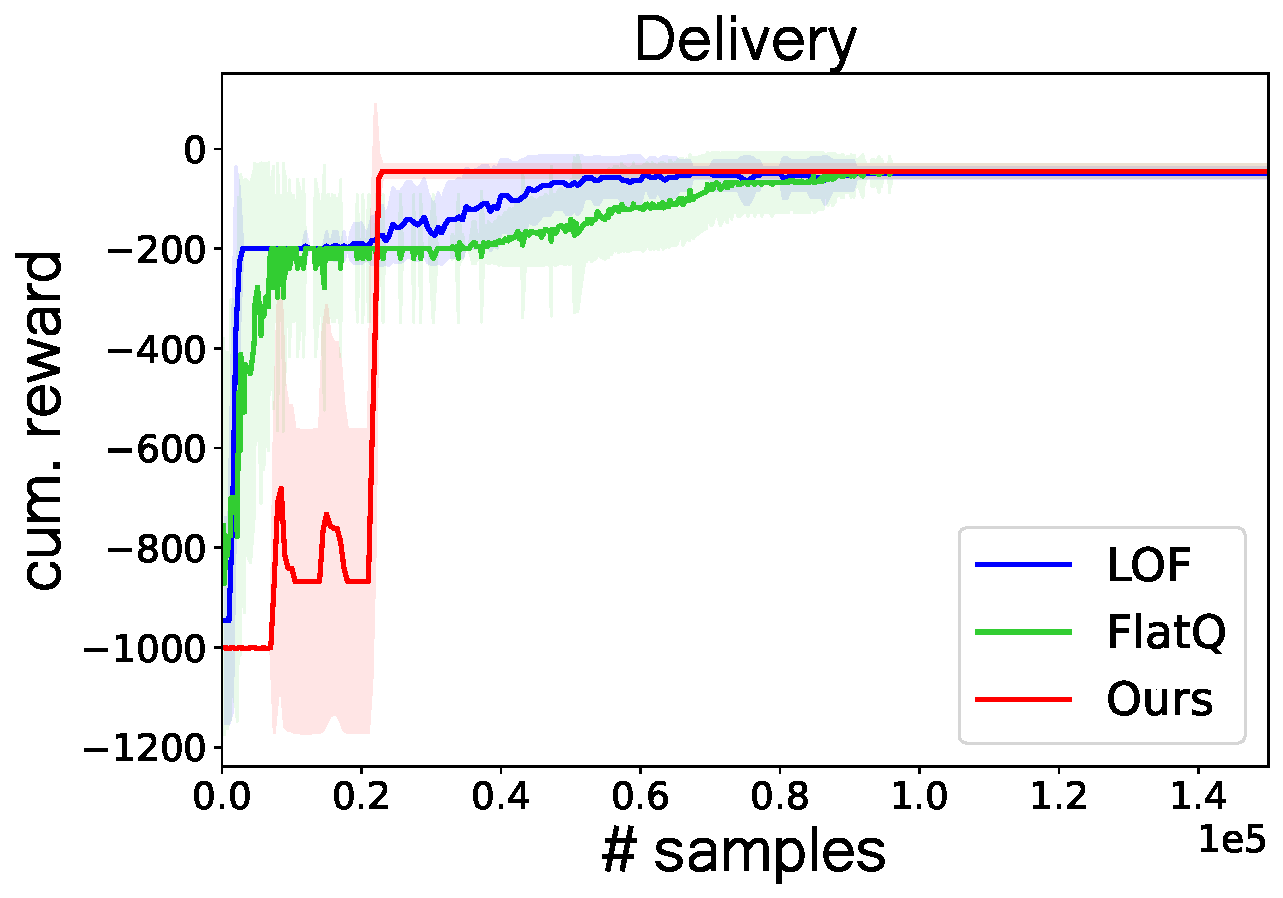
\includegraphics[scale=0.28]{figures/chapter3/results/delivery_learning.pdf}  
    % \subcaption{}
    % \label{fig:results1}
  \end{subfigure}
  \hfill
   \begin{subfigure}[t]{0.5\textwidth}
    \centering
    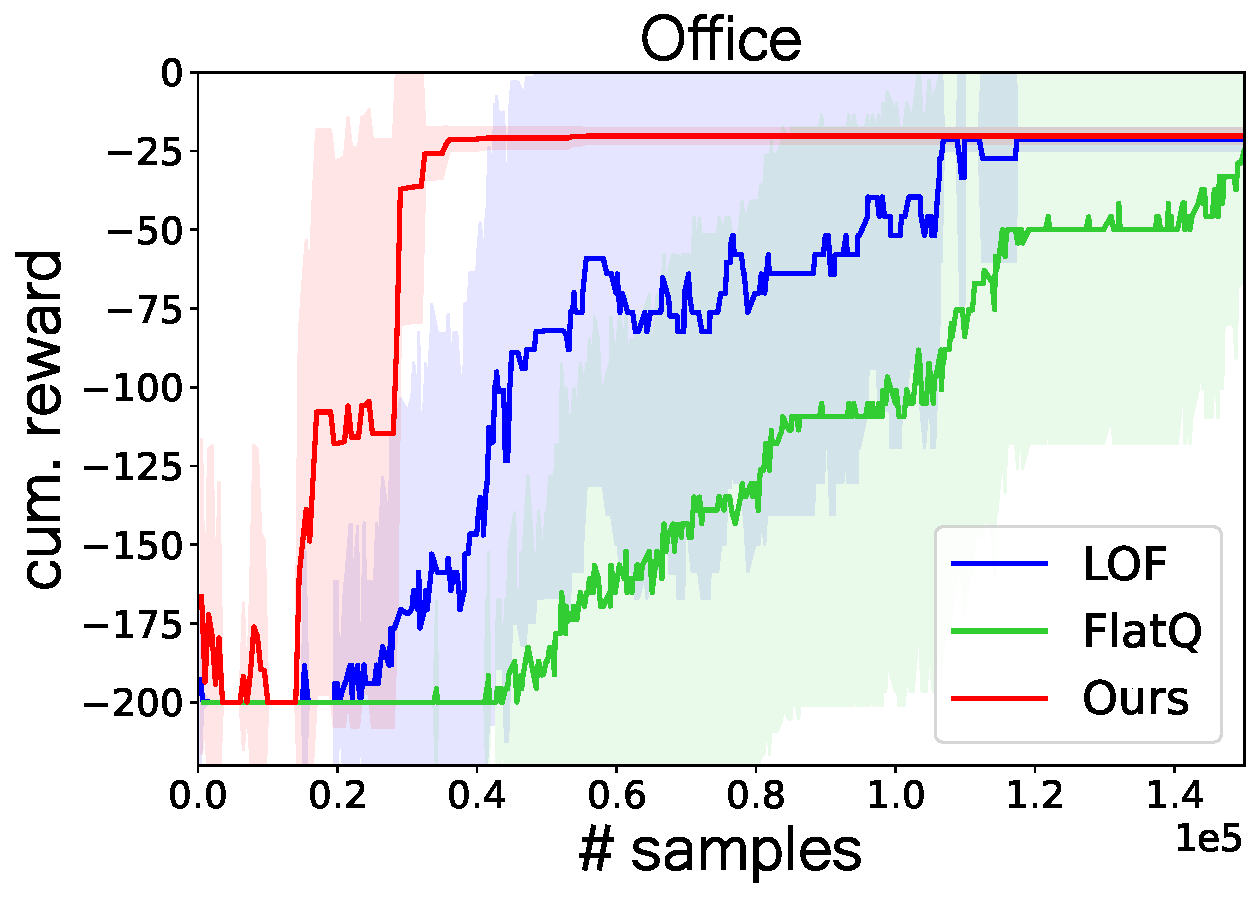
\includegraphics[scale=0.28]{figures/chapter3/results/office_learning.pdf}  
    % \subcaption{}
    % \label{fig:results2}
  \end{subfigure}
   \begin{subfigure}[b]{0.5\textwidth}
    \centering
    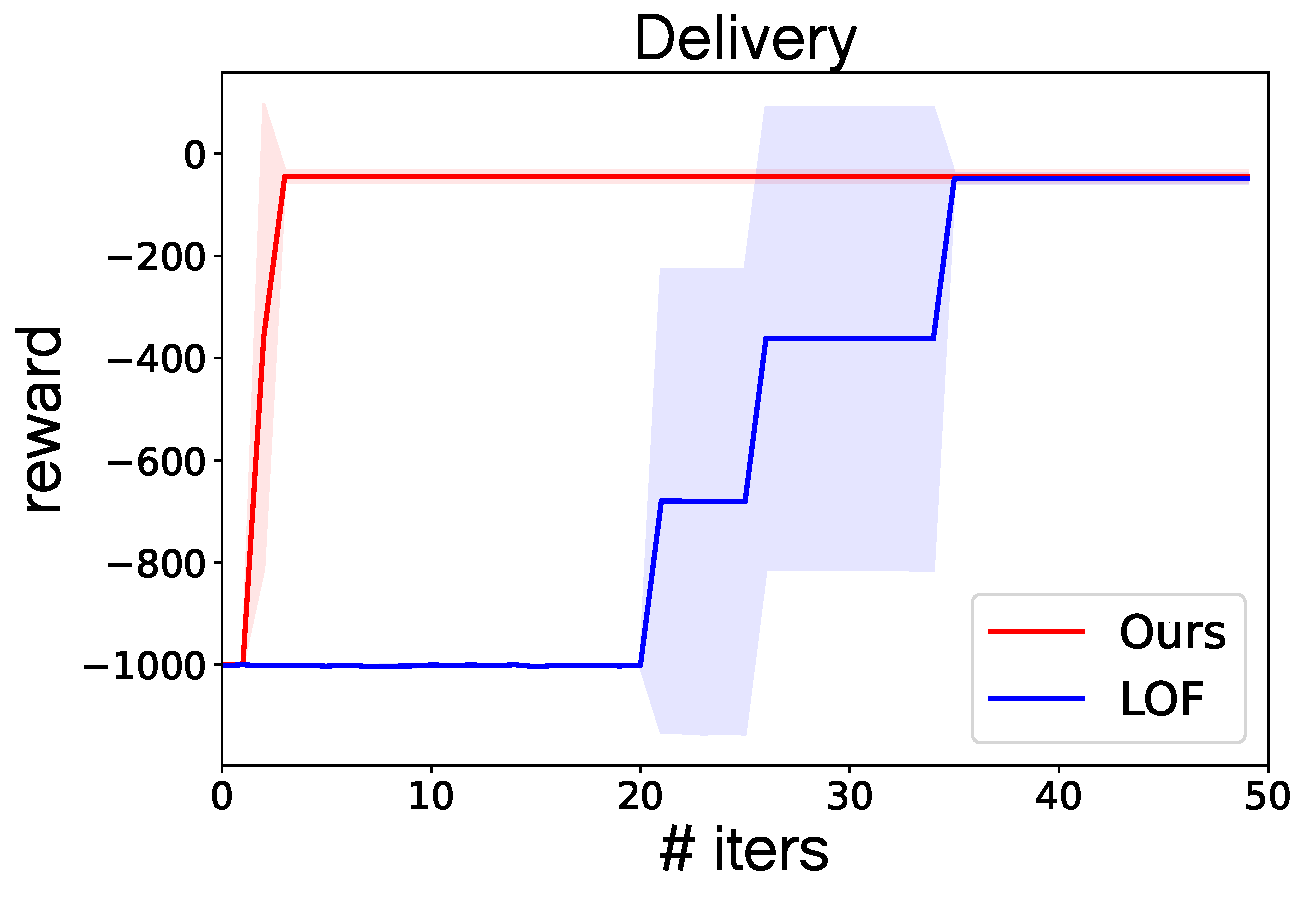
\includegraphics[scale=0.28]{figures/chapter3/results/readapt_delivery.pdf}  
    % \subcaption{}
    % \label{fig:results3}
  \end{subfigure}
  \hfill
   \begin{subfigure}[b]{0.5\textwidth}
    \centering
    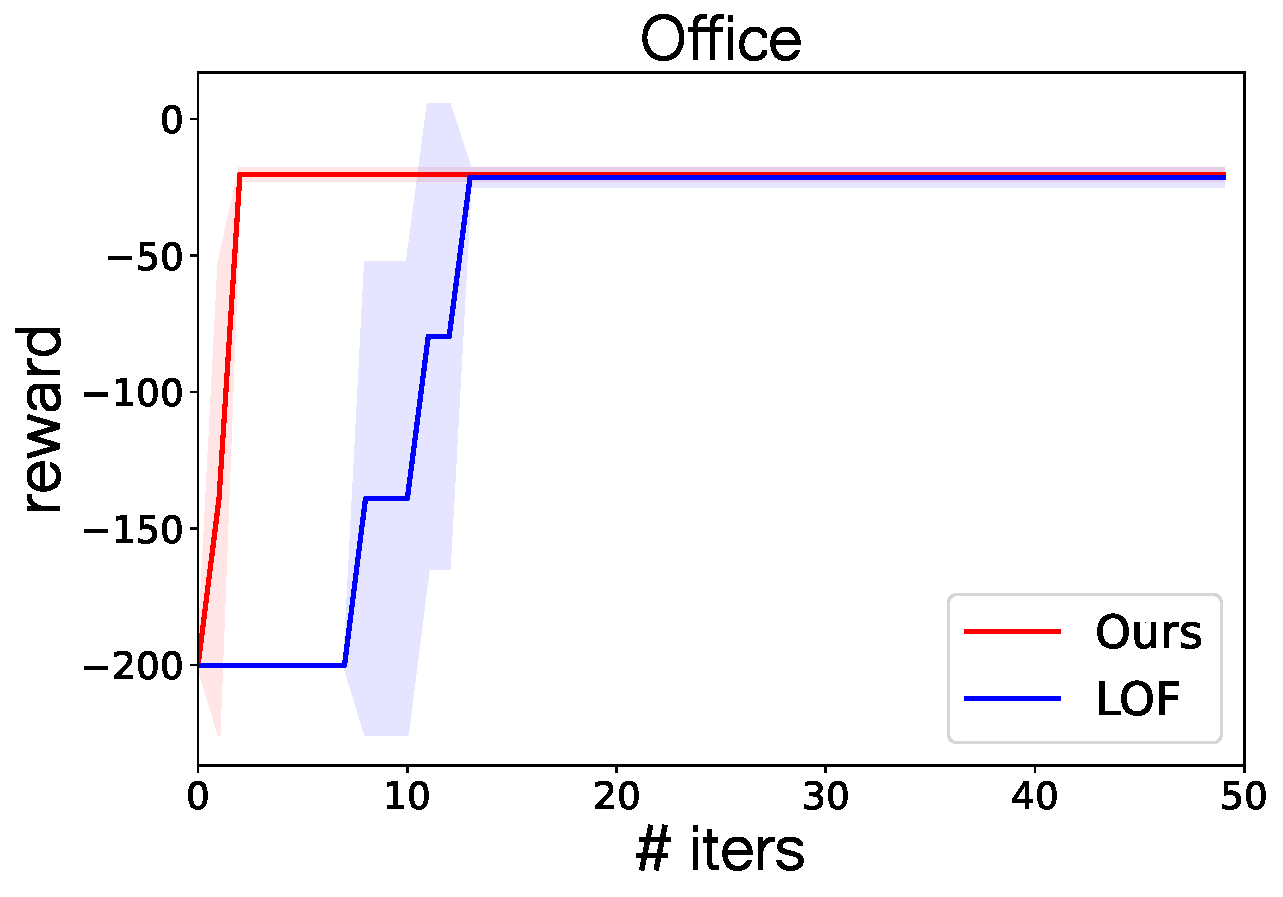
\includegraphics[scale=0.28]{figures/chapter3/results/readapt_office.pdf}  
    % \subcaption{}
    % \label{fig:results4}
  \end{subfigure}
  \caption{Experimental results for learning (Delivery, top-left and Office, bottom-left) and compositionality (Delivery, top-right and Office, bottom-right). Results show the average performance and standard deviation over the three tasks and 5 seeds per task.}
  \label{fig:exp_results}
\end{figure*}
\textsc{sf-fsa-vi} is tested in three complex discrete environments later described. At test time, the reward is changed to return $-1$ for every timestep and use the cumulative reward as the performance metric. This reward function effectively captures the number of steps to complete each task. Two types of results are reported. First, an important aspect is to observe the performance of the derived optimal policy, in Equation~\eqref{eq:hl-policy}, during the \textbf{learning} phase. For this, the high-level policy is fully retrained (lines 2-6 in Algorithm~\ref{alg:online}) every several learning interactions with the environment as $\Pi_\text{CCS}$ is being computed. Second, once the base behaviors are learned (this is once a complete $\Pi_\text{CCS}$ has been computed), the number of \textbf{planning} iterations \textsc{sf-fsa-vi} needs to converge to an optimal solution is measured for different task specifications. In both cases, results are compared against similar baselines.

\subsection{Environments and tasks} 

\paragraph{Office} A simplified version of the original Office domain~\citep{Icarte2018b} is used. In the context of this work, this is a complex environment since there are three propositional symbols $\cP=\{\text{\coffee}, \text{\mail}, o\}$ which can be satisfied at different locations, namely $\cE=\{\text{\coffee}^1, \text{\coffee}^2, \text{\mail}^1, \text{\mail}^1, o^1, o^2\}$. Here, there are no obstacle states and $\boldsymbol{\phi}(s,a,s')=\mathbf{0}\in\real^6$ for non-terminal transitions.

\paragraph{Delivery} In the Delivery domain~\citep{Araki2021}, shown in Figure~\ref{fig:delivery}, the set of exit states is ${\cE=\{A,B,C,H\}}$ while the propositonal symbol are $\cP=\{A,B,C,H,\blacksquare\}$. This means that features vectors are $\boldsymbol{\phi}(s,a,s')\in\real^5$. There are four symbols that are satisfied at the corresponding exit states, the feature vector for trainstions into these exit states correspond to the one-hot encodings of the terminal states. Additionally, there exist a propositional symbol $\blacksquare$ that represents an obstacle. Upon entering one of these states the corresponding feature vector component gets a value of $-1$. When solving an FSA, the weight of this symbol can be set to $\w_\blacksquare=1000$ which in practice corresponds to a very large negative reward. For regular states (in white in Figure~\ref{fig:delivery}), the feature vector is $\mathbf{0}\in\real^5$.


\begin{figure*}[!tb]
    \centering
    
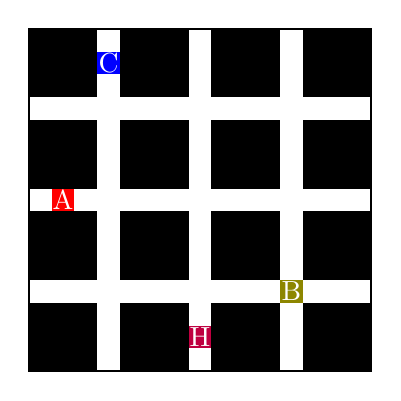
\begin{tikzpicture}[scale=0.29]
    % grid
    %\draw[step=1cm,gray] (0,0) grid (15, 15);
    % walls
    \fill[black] (0,0) rectangle ++ (3,3); 
    \fill[black] (4,0) rectangle ++ (3,3); 
    \fill[black] (8,0) rectangle ++ (3,3); 
    \fill[black] (12,0) rectangle ++ (3,3); 

    \fill[black] (0,4) rectangle ++ (3,3); 
    \fill[black] (4,4) rectangle ++ (3,3); 
    \fill[black] (8,4) rectangle ++ (3,3); 
    \fill[black] (12,4) rectangle ++ (3,3);

    \fill[black] (0,4) rectangle ++ (3,3); 
    \fill[black] (4,4) rectangle ++ (3,3); 
    \fill[black] (8,4) rectangle ++ (3,3); 
    \fill[black] (12,4) rectangle ++ (3,3);

    \fill[black] (0,8) rectangle ++ (3,3); 
    \fill[black] (4,8) rectangle ++ (3,3); 
    \fill[black] (8,8) rectangle ++ (3,3); 
    \fill[black] (12,8) rectangle ++ (3,3);

    \fill[black] (0,12) rectangle ++ (3,3); 
    \fill[black] (4,12) rectangle ++ (3,3); 
    \fill[black] (8,12) rectangle ++ (3,3); 
    \fill[black] (12,12) rectangle ++ (3,3);

    \fill[red] (1,7) rectangle ++ (1,1);
    \node at (1.5,7.5) {\color{white} A};
    \fill[blue] (3,13) rectangle ++ (1,1);
    \node at (3.5,13.5) {\color{white} C};
    \fill[olive] (11,3) rectangle ++ (1,1);
    \node at (11.5,3.5) {\color{white} B};
    \fill[purple] (7,1) rectangle ++ (1,1);
    \node at (7.5,1.5) {\color{white} H};

    % Symbols

    % agent
    % \node at (3.5,1.5) {\agent};
    % \draw[ultra thick, ->, >=stealth, draw=blue!70!white] (2.5,1.9) -- (2.5,2.5) -- (1.5,2.5) -- (1.5,3.5) -- (2.5,3.5) -- (2.5,5.5) -- (1.5,5.5) -- (1.5,6.5) -- (2.5,6.5) -- (2.5,7.5) -- (3.5,7.5) -- (3.5,6.8);
    % \draw[ultra thick, ->, >=stealth, draw=blue!70!white] (3.8,6.5) -- (4.3,6.5) -- (4.3,4.8);

    % Outer box
    \draw[ thick] (0,0) rectangle (15,15);

\end{tikzpicture}
  \caption{Depiction of the Office (a) and Delivery (b) environments, FSA task specification of the composite task in the Office domain and the FSA task specificiation of the sequential task in the Delivery domain (b). In (a) $\cP=\{\text{\coffee}, \text{\mail}, o\}$ and $\cE=\{\text{\coffee}^1,\text{\coffee}^2, \text{\mail}^1,\text{\mail}^2, o^1, o^2\}$. In (b), $\cE=\cP=\{A, B, C, H\}$.}
 \label{fig:delivery}
\end{figure*}

For each of the environments we define three different tasks: sequential, disjunction and composite (all described in the Supplementary Material). The sequential task is meant to show how our algorithm can indeed be effectively used to plan over long horizons, when the other two tasks show the ability of our method to optimally compose the base (sub)policies in complex settings. In natural language, the tasks in the Delivery domain correspond to: "go to $A$, then $B$, then $C$ and finally $H$"  (sequential), "go to $A$ or $B$, then $C$ and finally $H$" (disjunction) and "go to $A$ and $B$ in any order, then $B$, then $C$ and finally $H$" (composite). The agent has to complete the tasks by avoiding obstacles. The counterpart of these tasks in the Office environment are: "get a coffee, then pick up mail and then go to an office" (sequential), "get a coffee or mail, and then go to an office" (disjunction) and "get a coffee and mail in any order, and then go to an office" (composite). 
Our agent never learns how to solve these tasks, but rather learns the set of (sub)policies that constitutes the CCS. At test time, we provide the agent with the FSA task specification, extract a high-level optimal policy and test its performance on solving the task.

\subsection{Baselines} The logical options framework (\textsc{lof}, \citet{Araki2021}) highlights three desirable properties that hierarchical planning approaches should have: satisfaction, optimality and composability. All of these are satisfied by \textsc{sf-fsa-vi}. Thus, \textsc{lof} is used as a hierarchical baselines. \textsc{\textsc{lof}} trains one option per exit state, which are trained simultaneously using intra-option learning, and then uses a high-level value iteration algorithm to train a meta-policy that decides which option to execute in each of the MDP states. The implementation of \textsc{lof} used for the experiments follows the description given by the authors. The other baseline is Q-learning on the flat product MDP. Under certain conditions, flat Q-learning converges to the optimal value function but, especially for longer tasks, it may take a large number of samples and it is expected to perform worse than any of the hierarchical alternatives. Additionally, it is trained for a specific task, so it is not able to generalize to other task specifications. 

\subsection{Results}

\begin{figure}[!htb]
  \centering
  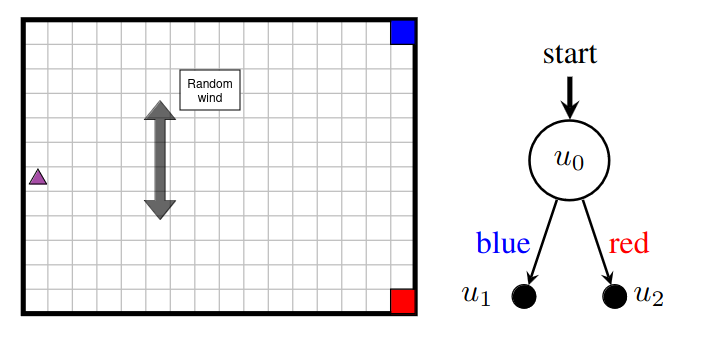
\includegraphics[width=0.7\textwidth]{figures/chapter3/double_slit.png}
  \caption{Double slit environment (right) and FSA to achieve either of the goal states ({\color{blue}blue} or {\color{red}red}) (left.)}
  \label{fig:double_slit}
\end{figure}

\paragraph{A motivating example} As it is shown later in the experimental results, in deterministic environments, it may suffice to learn a single (sub)policy (or option) per exit state to find an optimal policy via planning. In such cases, it may not be necessary to learn a full CCS. That is why, approaches that use the options framework such as \textsc{lof} traditionally define one option per subgoal. However, there are scenarios, in which these approaches will not find an optimal policy. This is the case for most stochastic environments. For example, consider the very simple domain of Double Slit in and the FSA task specification in Figure~\ref{fig:double_slit}. In this environment, there are two exit states $\cE=\{{\color{blue} \text{blue}}, {\color{red}\text{red}}\}$. The agent starts in the leftmost column and middle row. At every timestep, the agent chooses an action amongst $\{\text{UP}, \text{RIGHT}, \text{DOWN}\}$ and is pushed one column to the right in addition to moving in the chosen direction, except in the last column. If the agent chooses RIGHT, it moves an extra column to the right. At every timestep there is a random wind that can blow the agent away up to three positions in the vertical direction. The FSA task specification represents a task which is indifferently satisfied at either of the subgoal states. Note that this is indeed a Markovian reward specification. Since the RIGHT action brings the agent closer to both goals, the optimal behavior in this case is to commit to either goal as late as possible. In this setting, methods that use one policy per subgoal, such as \textsc{lof}, train two policies to reach both goals. This means that the agent has to commit to one of the goals from the very beginning, which hurts the performance as it has to make up for the consequences of the random noise. On the other hand, the CCS used by \textsc{sf-fsa-vi} will contain an additional policy that is indifferent to both subgoals goals. This leads to a performance gap as our approach achieves an average accumulated reward of $-19.7\pm3.65$ and \textsc{lof} $-22.70\pm 5.72$.

\paragraph{Learning} Empirical results for learning are shown in Figure~\ref{fig:exp_results} (top-left and bottom-left). The plots reflect how the different methods (ours, \textsc{lof} and flat Q-learning) perform at solving an FSA task specification during the learning phase. In the case of \textsc{sf-fsa-vi} and \textsc{lof}, the learning phase corresponds to obtaining the low level (sub)policies for $\Pi_\text{CCS}$ and the options, while for . Results are averaged over the three tasks (sequential, disjunction and composite) previously described for each environment. Each data point in the plots represent the cumulative reward obtained by a fully retrained policy with the current status of $\Pi_\text{CCS}$ and options. In both environments, \textsc{sf-fsa-vi} is the first to reach optimal performance. There exist, however, some differences between \textsc{lof} and \textsc{sf-fsa-vi}. \textsc{lof} trains all options simultaneously with intra-option learning. This means that, every transition $(s_t, a_t, s_{t+1})$ is used to update all options' value functions and policies. The learning of a $\Pi_\text{CCS}$, on the other hand, is done sequentially. A fixed sample budget per (sub)policy is set prior to learning, which can be seen as a hyperparameter. We use a total of $8\cdot 10^3$ samples per (sub)policy in both environments. A experience replay buffer is used to speed up the learning of the policy basis $\Pi_\text{CCS}$. Both options and the SF representation of (sub)policies are learned using Q-learning. Due to the incremental nature, at the beginning of the learning process there might be not enough policies in the basis $\Pi_\text{CCS}$ to construct a feasible solution. This is clearly observed in the Delivery domain (Figure~\ref{fig:exp_results}, top left), where at the early stages of the interaction, \textsc{sf-fsa-vi} achieves very low cumulative reward due to failing at delivering a solution. It is not until when there are enough (sub)policies in the basis that Algorithm~\ref{alg:online} attains a policy that solves the problem, which eventually converges to an optimal policy. Similarly, \textsc{lof} converges to an optimal policy albeit it takes slightly longer to learn. In the more complex Office environment, results follow the same pattern. However, this environment breaks one of the of \textsc{lof} requirements for optimality: to have a single exit state associated with each propositional predicate. In this problem, for each predicate there exist two exit states that can satisfy them. This makes \textsc{lof} prone to converge to suboptimal solutions when \textsc{sf-fsa-vi} attains optimality. This is the case for the composite task, where \textsc{lof} is short-sighted and returns a longer path (in red, Figure~\ref{fig:office_env}) in contrast to ours that retrieves the optimal solution (in green, Figure~\ref{fig:office_env}). This means that \textsc{sf-fsa-vi} is more flexible in the task specification. In this environment, our algorithm also converges faster with a more obvious gap with respect to \textsc{lof}. In any case, learning (sub)policies or options is faster than learning directly on the flat product MDP, as flat Q-learning takes the longest to converge.

\paragraph{Planning} Figure~\ref{fig:exp_results} top-right and bottom-right show how fast \textsc{sf-fsa-vi} and \textsc{lof} can plan for an optimal solution. Results are again averaged for the three tasks for each environment. Here, a complete policy basis $\Pi_\text{CCS}$ has been previously computed, as well as the option's optimal policies.  In \textsc{lof}, the cost of each iteration of value iteration is $\lvert\cU\rvert\times\lvert\cS\rvert\times \lvert\cK\rvert$, where $\cK$ is the set of options, while for the Algorithm~\ref{alg:online} we propose it is $\lvert\cU\rvert\times\lvert\cE\rvert\times\lvert\Pi_\text{CCS}\rvert$. By definition, the number of options is equivalent to the number of exit states $\lvert\cK\rvert=\lvert\cE\rvert$, so a single iteration of \textsc{sf-fsa-vi} is more efficient than \textsc{lof} whenever $\lvert\Pi_\text{CCS}\rvert \ll \lvert\cS\rvert$. In our experiments, the sizes of the CCS are $15$ and $12$ for the Delivery and Office domains, respectively, while the sizes of the state spaces are of $225$ and $121$. Therefore, since our algorithm needs fewer, shorter iterations during planning, it outperforms \textsc{lof} in terms of planning speed in both domains when composing the global solution. This can be observed in the plots for both environments. 

% \begin{figure}[!htb]
%   \centering
%   \begin{subfigure}[t]{0.23\textwidth}
%     \centering
%     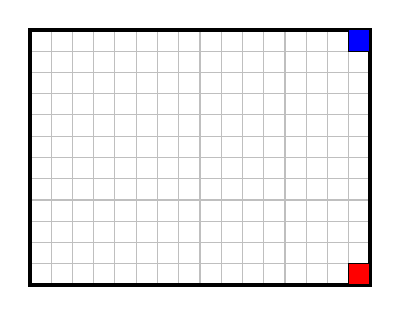
\begin{tikzpicture}[scale=0.54]

    % Outer box
    \draw[step=0.5cm,lightgray] (0,0) grid (8, 6);
    \draw[ultra thick] (0,0) rectangle (8,6);

    % agent
    \node at (0.3, 2.8) {\miniagent};
    % \draw[ultra thick, ->, >=stealth, draw=blue!70!white] (2.5,1.9) -- (2.5,2.5) -- (1.5,2.5) -- (1.5,3.5) -- (2.5,3.5) -- (2.5,5.5) -- (1.5,5.5) -- (1.5,6.5) -- (2.5,6.5) -- (2.5,7.5) -- (3.5,7.5) -- (3.5,6.8);
    % \draw[ultra thick, ->, >=stealth, draw=blue!70!white] (3.8,6.5) -- (4.3,6.5) -- (4.3,4.8);
    \draw[fill=blue] (7.5,5.5) --  (7.5,6) -- (8,6) -- (8,5.5) -- cycle;
    % Outer box
    \draw[fill=red]  (7.5,0) --  (7.5,0.5) -- (8,0.5) -- (8,0) -- cycle;

    % \node[color=white] at (7.5,5.5) {$\text{G}_1$};
    % \node[color=white] at (7.5,0.5) {$\text{G}_2$};

\end{tikzpicture}

%   \end{subfigure}
%   \hfill
%   \begin{subfigure}[t]{0.23\textwidth}
%     \centering
%     \begin{tikzpicture}[node distance=cm,on grid,every initial by arrow/.style={ultra thick,->, >=stealth}]
    \node[thick,state,initial above] (u_0) at (0,0) {$u_0$};
    % \node[circle,draw=black,minimum size=0.26cm,inner sep=0pt,fill=black] (t1) at (2,0)  {};
    % \node[circle,draw=black,minimum size=0.26cm,inner sep=0pt,fill=black] (t2) at (2,-1.8)  {};
    \node[circle,draw=black,minimum size=0.26cm,inner sep=0pt,fill=black] (t1) at (-0.5,-1.5)  {};
    \node[circle,draw=black,minimum size=0.26cm,inner sep=0pt,fill=black] (t2) at (0.5,-1.5)  {};
    \node[text width=1cm ] at (-0.7,-1.5) {$u_1$};
    \node[text width=1cm ] at (1.2,-1.5) {$u_2$};
    \path[thick,->, >=stealth] (u_0) edge node [left] {\color{blue} blue} (t1);
    \path[thick,->, >=stealth] (u_0) edge node [right] {\color{red} red} (t2);
    %\path[ultra thick,->, >=stealth] (q_0) edge [loop left] node {$\tuple{\neg \text{\coffee},0}$} ();
    % \path[ultra thick,->, >=stealth] (q_0) edge node [above] {$\tuple{\text{\decoration},0}$} (t1);
    %\path[ultra thick,->, >=stealth] (q_1) edge [loop left] node {$\tuple{\neg o,0}$} ();
    % \path[ultra thick,->, >=stealth] (q_1) edge node [above] {$\tuple{\text{\decoration},0}$} (t2);
    %\path[ultra thick,->, >=stealth] (u_1) edge node [above]{$o$} (t3);
\end{tikzpicture}
%   \end{subfigure}
%   \caption{Double Slit environment (left) and FSA task specification to reach either goal locations {\color{blue}blue} or {\color{red}red}.}
%  \label{fig:double_slit}
% \end{figure} 

\section{Related Work}
One of the key distinctions of this work compared to prior studies is the optimality of the final solution. As noted by \citep{Dietterich2000}, hierarchical methods usually have the capability to achieve hierarchical, recursive, or global optimality. The challenge that often arises when subtask policies are trained in isolation is that the combination of these locally optimal policies does not lead to a globally optimal policy but a recursively \citep{Dayan1992} or hierarchically optimal policy \citep{Sutton1999, Mann2015, Araki2021}.  To tackle this challenge, our approach relies on acquiring a set of low-level policies for each subtask and employing planning to identify the optimal combination of low-level policies when solving a particular task. By learning the CCS with OLS \citep{Roijers2014} in combination with high-level planning, \textsc{sf-fsa-vi} ensures that globally optimal policy is achieved. In this regard, the work of \citep{Alegre2022} is of particular interest as it was the first work that used OLS and successor features \textit{Barreto2017} for optimal policy transfer learning. However, this method has only applied in a setting with Markovian reward function and has not been used with non-Markovian task specifications or high-level planning. 

On the other hand, many recent approaches proposed to use high-level task specifications in the form of LTL~\citep{Icarte2018b, Kuo2020, Vaezipoor2021, Jothimurugan2021}, or similar formal language specifications~\citep{ToroIcarte2019,Camacho2019, Araki2021, Icarte2022} to learn policies. However, the majority of the methods in this area are designed for single-task solutions, with only several focusing on acquiring a set of policies that is capable of addressing multiple tasks \citep{Icarte2018b, Leon2020, Kuo2020, Araki2021, Vaezipoor2021}. Nonetheless, these approaches cannot guarantee optimality.

From these works, our approach is the most similar to the logical options framework (\textsc{lof}, \citet{Araki2021}). The main difference is that \textsc{lof} trains a single policy for each subgoal, resulting in a set of learned policies that is either smaller than or equal to the set acquired through \textsc{sf-fsa-vi}. While employing one policy per subgoal proves sufficient for obtaining a globally optimal policy through planning in deterministic environments~\citep{Wen2020}, this may not hold true in stochastic environments, as our experiments demonstrate. In such instances, the policies generated by \textsc{lof} are hierarchically optimal but fall short of global optimality.


Two notable examples from aforementioned works on multi-task learning with formal language specifications are the works of \citep{Icarte2018b} and \citep{Vaezipoor2021}. The former struggles with generalizing to unseen tasks, because it uses LTL progression to determine which subtasks need to be learned to solve given tasks. The Q-functions that are subsequently learned for each LTL subtask will therefore not be useful for a new task if its subtasks were not part of the training set. Such limitation does not apply to the latter as it instead encodes the remaining LTL task specification using a neural network and conditions the policy on this LTL embedding. While this approach may be more adaptable to tasks with numerous propositions or subgoals, it risks generating sub-optimal policies as it relies solely on the neural network to select the next proposition to achieve, without incorporating planning. Additionally, since the planning is implicitly done by the neural network, the policy is less interpretable than when explicit planning is used.

The method we propose can be viewed as a method for composing value functions through successor features, akin to previously proposed approaches for composition of value functions and policies ~\citep{Niekerk2019, Barreto2019, NangueTasse2020, Infante2022}. In the work of ~\citep{Infante2022}, which is the closest to our work, the authors propose to learn a basis of value functions that can be combined to form an optimal policy. However, unlike \textsc{sf-fsa-vi}, their approach only works in a restricted class of linearly-solvable MDPs. Lastly, since our approach uses the values of exit states for planning it is also related to planning with exit profiles \citep{Wen2020}. The CCS that we propose to use as a policy basis in our work can be seen as a collection of policies that are optimal for all possible exit profiles.

\section{Discussion and Conclusion}

In this work, we address the problem of finding optimal behavior for new non-Markovian goal specifications in known environments. To do so, we introduce a novel approach that uses successor features to learn a policy basis, that can subsequently be used to solve any unseen task specified by an FSA with the set of given predicates $\cP$ by planning. \textsc{sf-fsa-vi} is the first that can provably generalize to such new task specification without sacrificing optimality in both deterministic and stochastic environments.

The experiments show that \textsc{sf-fsa-vi} offers several advantages over previous methods. First, due to the use of SF, it allows for faster composition of the high-level value function since it drastically reduces the number of states to plan on. Secondly, thanks to using a CCS over a set of options \textsc{sf-fsa-vi} achieves optimality even in stochastic environments (as shown in the Double Slit example). Lastly, we do not require that there exists a single exit state per predicate which permits more flexible task specification while at the same time allowing deployment in more complex environments. 

A limitation of our approach could be the need to construct a full CCS if one wants to attain global optimality. While the construction of CCS is not timecomsuming for environments with several exit states presented in our work, the computation cost of finding the full CCS could become too large for environments with many exit states. In such case one could instead learn a partial CCS at the cost of a bounded decrease in performance \citep{Alegre2022} or consider splitting the environment into smaller parts with fewer exit states. While our experiments only considered discrete environments, \textsc{sf-fsa-vi} should also be applicable in continuous environments with minor adjustments. These include: using an contiguous set of states instead of a single exit state and using reward shaping to facilitate learning in sparse reward setting.